\begin{figure}[!htbp]
\centering
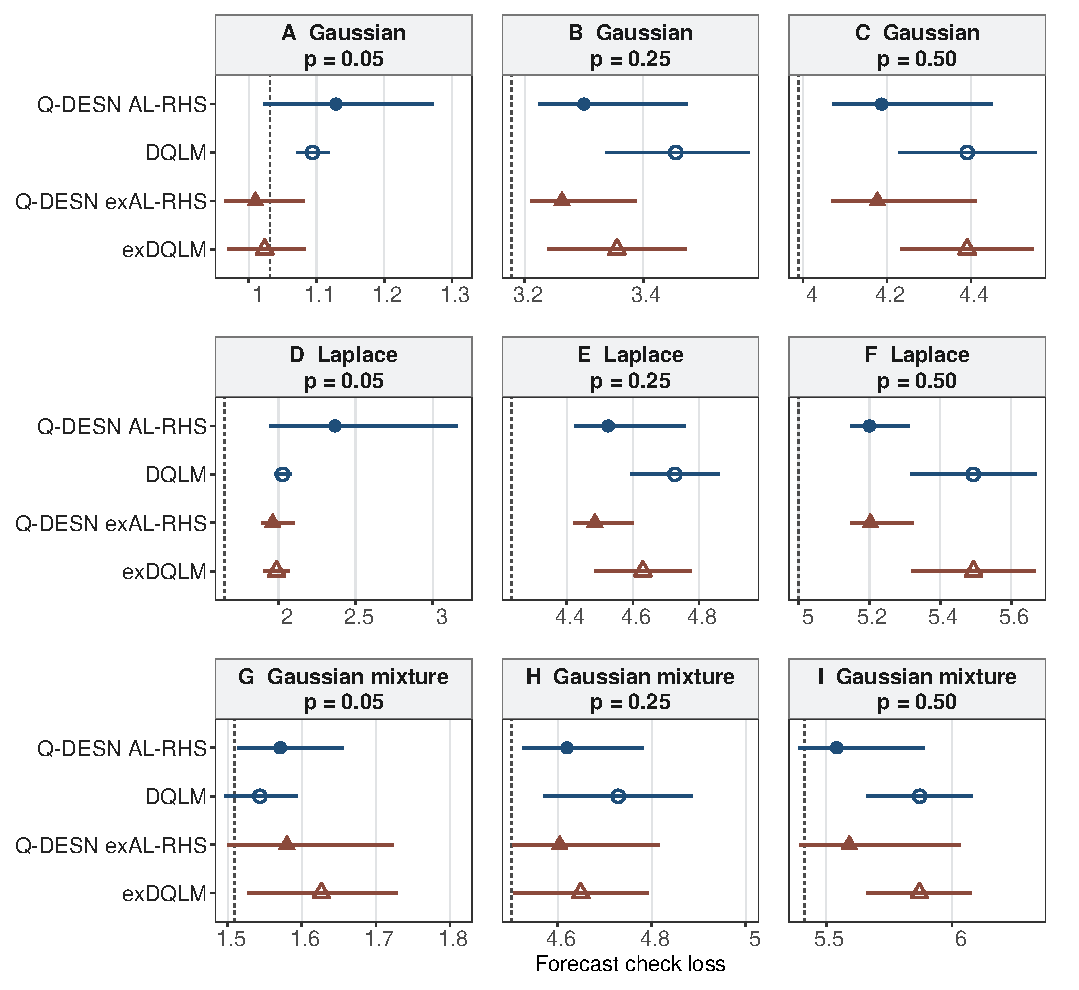
\includegraphics[width=0.98\textwidth]{figures/independent_simulation/independent_train500_eval300_mcmc_forecast_check_v1.pdf}
\caption{MCMC forecast check loss over the first 300 evaluation targets (10 origins). Points and equal-tailed 95\% intervals summarize the draw-wise criterion averaged over scored pairs; lower is better. Navy circles identify \(\AL\) models and muted-brick triangles \(\exAL\) models; filled symbols denote Q--DESN and open symbols their dynamic linear comparators. Panels A--I identify the observation-error family and probability level. The dashed line marks population expected check loss at the true conditional quantile, not a finite-sample lower bound. Panel scales match the 500-target sensitivity figures. The supplement documents criterion-specific selection and model-specific forecast-draw dependence.}
\figalt{Nine panels compare four models using mean forecast check loss and 95 percent intervals over 300 scored targets.}
\label{fig:simulation-500obs-mcmc-forecast-check-loss-intervals}
\end{figure}
